\subsubsection{MainLayout}

\begin{center}
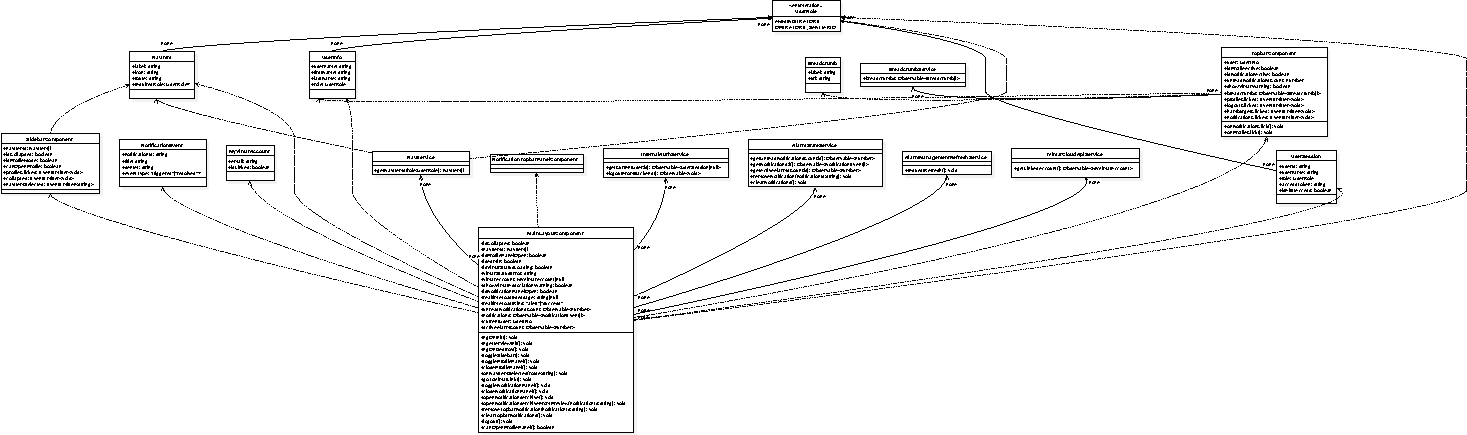
\includegraphics[width=\textwidth]{./frontend/mainLayout/main-layout.pdf}
\captionof{figure}{Diagramma delle classi del modulo MainLayout}
\end{center}


\addAtr{+}{topbarRef: ElementRef}{Riferimento all'elemento DOM della topbar per osservazioni di resize.}
\addAtr{+}{isCollapsed: boolean}{Indica se la sidebar è collassata o espansa.}
\addAtr{+}{navItems: NavItem[]}{Array degli elementi di navigazione basati sul ruolo utente.}
\addAtr{+}{isProfilePanelOpen: boolean}{Indica se il pannello del profilo è aperto.}
\addAtr{+}{isAdmin: boolean}{Indica se l'utente corrente ha ruolo amministratore.}
\addAtr{+}{isVimarStatusLoading: boolean}{Indica se il caricamento dello stato Vimar è in corso.}
\addAtr{+}{vimarStatusError: string}{Messaggio di errore relativo allo stato del collegamento Vimar.}
\addAtr{+}{vimarAccount: MyVimarAccount $|$ null}{Account Vimar collegato o null se non disponibile.}
\addAtr{+}{showVimarAssociationWarning: boolean}{Indica se mostrare l'avviso di associazione Vimar.}
\addAtr{+}{isNotificationPanelOpen: boolean}{Indica se il pannello delle notifiche è aperto.}
\addAtr{+}{realtimeToastMessage: string $|$ null}{Messaggio del toast in tempo reale o null se non presente.}
\addAtr{+}{realtimeToastKind: 'alert' $|$ 'success'}{Tipo del toast in tempo reale, alert o success.}
\addAtr{-}{navService: NavService}{Servizio per gestire gli elementi di navigazione.}
\addAtr{-}{internalAuthService: InternalAuthService}{Servizio per l'autenticazione interna.}
\addAtr{-}{alarmStateService: AlarmStateService}{Servizio per lo stato degli allarmi e notifiche.}
\addAtr{-}{alarmManagementRefreshService: AlarmManagementRefreshService}{Servizio per il refresh della gestione allarmi.}
\addAtr{-}{router: Router}{Router di Angular per la navigazione.}
\addAtr{-}{myVimarService: IVimarCloudApiService $|$ null}{Servizio API per MyVimar, opzionale.}
\addAtr{+}{unreadNotificationsCount\$: Observable$<$number$>$}{Observable del conteggio delle notifiche non lette.}
\addAtr{+}{notifications\$: Observable$<$NotificationEvent[]$>$}{Observable dell'array delle notifiche.}
\addAtr{-}{cdr: ChangeDetectorRef}{Riferimento al change detector per aggiornamenti manuali.}
\addAtr{-}{destroy\$: Subject$<$void$>$}{Subject per gestire la distruzione del componente.}
\addAtr{-}{toastTimer: ReturnType$<$typeof setTimeout$>$ $|$ null}{Timer per il toast in tempo reale.}
\addAtr{-}{latestRealtimeNotificationId: string $|$ null}{ID dell'ultima notifica in tempo reale ricevuta.}
\addAtr{+}{currentUser: UserInfo}{Informazioni dell'utente corrente.}
\addAtr{+}{activeAlarmCount\$: Observable$<$number$>$}{Observable del conteggio degli allarmi attivi.}
\addAtr{-}{resizeObserver: ResizeObserver}{Osservatore per i cambiamenti di dimensione della topbar.}
\addMet{+}{ngOnInit() : void}{Inizializza il componente, legando le notifiche e caricando i dati utente.}
\addMet{+}{ngAfterViewInit() : void}{Dopo l'inizializzazione della vista, osserva le dimensioni della topbar.}
\addMet{+}{ngOnDestroy() : void}{Distrugge il componente, completando i subject e disconnettendo l'osservatore.}
\addMet{+}{toggleSidebar() : void}{Alterna lo stato di collasso della sidebar.}
\addMet{+}{toggleProfilePanel() : void}{Alterna l'apertura del pannello del profilo e carica lo stato Vimar se admin.}
\addMet{+}{closeProfilePanel() : void}{Chiude il pannello del profilo.}
\addMet{+}{onNavItemSelected(route: string) : void}{Gestisce la selezione di un elemento di navigazione, richiudendo pannelli e gestendo refresh.}
\addMet{+}{goToVimarLink() : void}{Naviga alla pagina di collegamento Vimar.}
\addMet{+}{toggleNotificationPanel() : void}{Alterna l'apertura del pannello delle notifiche.}
\addMet{+}{closeNotificationPanel() : void}{Chiude il pannello delle notifiche.}
\addMet{+}{openNotificationsArchive() : void}{Naviga all'archivio delle notifiche.}
\addMet{+}{openNotificationsArchiveFromPreview(notificationId: string) : void}{Naviga all'archivio notifiche focalizzandosi su una specifica notifica.}
\addMet{+}{removeTopbarNotification(notificationId: string) : void}{Rimuove una notifica dalla topbar tramite ID.}
\addMet{+}{clearTopbarNotifications() : void}{Cancella tutte le notifiche dalla topbar.}
\addMet{+}{logout() : void}{Effettua il logout, navigando alla pagina di login.}
\addMet{+}{canOpenProfilePanel() : boolean}{Verifica se il pannello del profilo può essere aperto.}
\addMet{-}{bindRealtimeAlarmNotifications() : void}{Collega le notifiche di allarme in tempo reale.}
\addMet{-}{openRealtimeNotificationPanel() : void}{Apre il pannello delle notifiche in tempo reale.}
\addMet{-}{showRealtimeToast(message: string, kind: 'alert' $|$ 'success') : void}{Mostra un toast in tempo reale con messaggio e tipo.}
\addMet{-}{clearToastTimer() : void}{Cancella il timer del toast in tempo reale.}
\addMet{-}{loadVimarStatus() : void}{Carica lo stato del collegamento Vimar, gestendo errori e caricamenti.}
\makeCl{MainLayoutComponent}{Il componente MainLayoutComponent gestisce il layout principale dell'applicazione, includendo sidebar, topbar e pannelli per profilo e notifiche. Coordina servizi per autenticazione, allarmi e navigazione, supportando funzionalità specifiche per amministratori come l'integrazione Vimar.}

\addAtr{+}{navItems: NavItem[]}{Array degli elementi di navigazione da visualizzare nella sidebar.}
\addAtr{+}{isCollapsed: boolean}{Indica se la sidebar è collassata o espansa.}
\addAtr{+}{isProfileMode: boolean}{Indica se la sidebar è in modalità profilo.}
\addAtr{+}{canOpenProfile: boolean}{Indica se è possibile aprire il pannello del profilo.}
\addAtr{+}{profileClicked: EventEmitter$<$void$>$}{Event emitter per notificare quando il profilo viene cliccato.}
\addAtr{+}{collapsed: EventEmitter$<$void$>$}{Event emitter per notificare quando la sidebar viene collassata.}
\addAtr{+}{navItemSelected: EventEmitter$<$string$>$}{Event emitter per notificare quando un elemento di navigazione viene selezionato.}
\makeCl{SidebarComponent}{Il componente SidebarComponent rappresenta il componente presentazionale della sidebar, visualizzando gli elementi di navigazione e gestendo le interazioni utente. Comunica con il componente padre tramite Input per i dati e Output per emettere i principali eventi di interazione.}

\addAtr{+}{user: UserInfo}{Informazioni dell'utente corrente da visualizzare nella topbar.}
\addAtr{+}{isProfileActive: boolean}{Indica se il pannello del profilo è attualmente attivo.}
\addAtr{+}{isNotificationActive: boolean}{Indica se il pannello delle notifiche è attualmente attivo.}
\addAtr{+}{unreadNotificationsCount: number}{Numero di notifiche non lette da visualizzare.}
\addAtr{+}{showVimarWarning: boolean}{Indica se visualizzare l'avviso di associazione Vimar.}
\addAtr{+}{profileClicked: EventEmitter$<$void$>$}{Event emitter per notificare quando il profilo viene cliccato.}
\addAtr{+}{logoutClicked: EventEmitter$<$void$>$}{Event emitter per notificare quando il logout viene cliccato.}
\addAtr{+}{hamburgerClicked: EventEmitter$<$void$>$}{Event emitter per notificare quando l'hamburger menu viene cliccato.}
\addAtr{+}{notificationClicked: EventEmitter$<$void$>$}{Event emitter per notificare quando le notifiche vengono cliccate.}
\addAtr{+}{breadcrumbs\$: Observable$<$Breadcrumb[]$>$}{Observable della lista di breadcrumb da visualizzare.}
\addAtr{-}{breadcrumbService: BreadcrumbService}{Servizio per gestire i breadcrumb della navigazione.}
\addMet{+}{onNotificationClick() : void}{Emette un evento quando l'utente clicca sull'icona delle notifiche.}
\addMet{+}{onProfileClick() : void}{Emette un evento quando l'utente clicca sull'icona del profilo.}
\makeCl{TopbarComponent}{Il componente TopbarComponent rappresenta la barra superiore dell'applicazione, visualizzando informazioni utente, conteggio notifiche, breadcrumb e icone di interazione. Comunica con il componente padre tramite Input per i dati e Output per emettere gli eventi di interazione dell'utente.}

\addMet{+}{getNavItems(role: UserRole) : NavItem[]}{Recupera la lista di elementi di navigazione filtrata in base al ruolo utente fornito, escludendo le opzioni riservate agli amministratori.}
\makeCl{NavService}{Il servizio NavService fornisce gli elementi di navigazione disponibili per l'utente, filtrando le opzioni in base al ruolo assegnato. Gestisce le autorizzazioni di accesso e le rotte associate a ciascun elemento di navigazione.}